\documentclass[tikz,border=5mm]{standalone}
\usetikzlibrary{patterns}
\begin{document}
	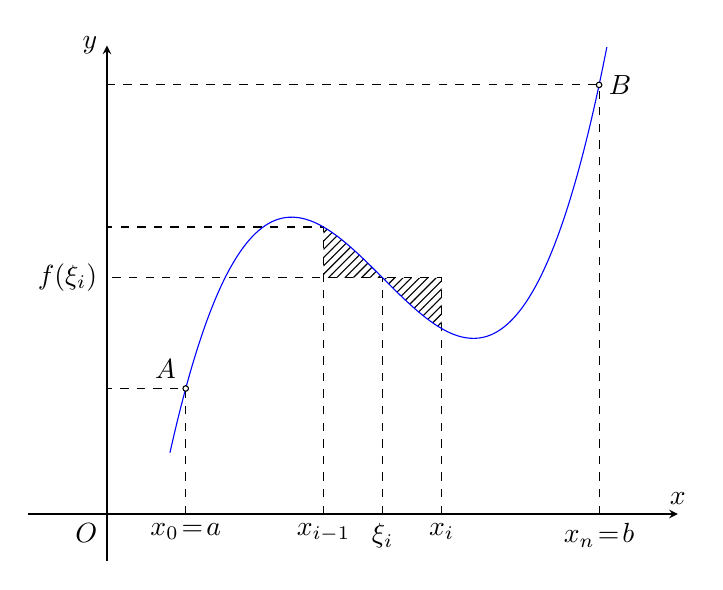
\begin{tikzpicture}[>=stealth]
		\def\f(#1){0.25*(#1-3.5)^3-(#1-3.5)+3}
		\def\a{1} \def\b{6.25}
		\def\m{2.75} \def\n{3.5} \def\p{4.25}
		\pgfmathsetmacro{\fa}{\f(\a)}
		\pgfmathsetmacro{\fm}{\f(\m)}
		\pgfmathsetmacro{\fn}{\f(\n)}
		\pgfmathsetmacro{\fp}{\f(\p)}
		\pgfmathsetmacro{\fb}{\f(\b)}
		\path[pattern=north east lines]
		plot[domain=\m:\n,smooth,samples=100] (\x,{\f(\x)})-|cycle
		plot[domain=\p:\n,smooth,samples=100] (\x,{\f(\x)})-|cycle;
		\draw[dashed]
		(\a,0)|-(0,\fa) (\b,0)|-(0,\fb)
		(\m,0)|-(0,\fm) (\n,0)|-(0,\fn) (\p,0)|-(\n,\fn);
		\draw[blue] plot[domain=\a-.2:\b+.1,smooth,samples=100] (\x,{\f(\x)});
		\draw[->] (-1,0)--(\b+1,0) node[above]{$x$};
		\draw[->] (0,-.6)--(0,\fb+.5) node[left]{$y$};
		\path
		(0,0) node[below left]{$O$}
		(\a,0) node[below]{$x_{0}\!=\!a$}
		(\m,0) node[below]{$x_{i-1}$}
		(\n,0) node[below]{$\xi_{i}$}
		(\p,0) node[below]{$x_{i}$}
		(\b,0) node[below]{$x_{n}\!=\!b$}
		(0,\fn) node[left]{$f(\xi_{i})$};
		\draw[fill=white]
		(\a,\fa) node[above left]{$A$} circle(1pt)
		(\b,\fb) node[right]{$B$} circle(1pt);
	\end{tikzpicture}
\end{document}